\chapter{METHODOLOGY}\label{chp:chapter3}
\thispagestyle{fancy}
The evaluation methodology is based on the injection of realistic vulnerabilities and the subsequent controlled exploit of those
vulnerabilities in order to attack the system. This provides a practical environment that can be used to test
counter measure mechanisms (such as IDS, web application vulnerability scanners, firewalls, etc.), train and evaluate security teams, estimate security measures (like the
number of vulnerabilities present in the code, in a similar
way to defect seeding  \cite{12}), among others.To obtain a realistic environment, true
to life vulnerabilities will be consider. As mentioned before,
results from a field study presented in [16] that classified
655 XSS and SQLi security patches of six widely used
LAMP web applications are utilized. This data will help to define
where a real vulnerability is usually located in the source
code and what is the piece of code that is responsible for the
presence of such vulnerability.\\
\newline
A typical web application is referenced , with a web front-end and an access to a back-end database to store the dynamic content and business data (Fig. 3.1).The vulnerabilities are injected in the web application following a realistic pattern . The information
about what was injected is fed to the injection mechanism in
order to improve the attack success rate.


\begin{figure} [H]
\centering
\fbox{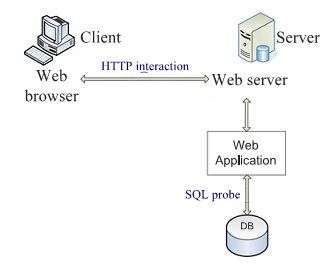
\includegraphics[width=0.65\linewidth]{Main/Fig1}}
\caption{A normal Web Application Setup}
\label{fig:Fig1}
\end{figure}

The attack injection tool uses two external
probes as shown in Fig 3.2: one for the HTTP communication and other for the
database communication.These probes monitor the HTTP
and SQL data exchanged, and send a copy to be analyzed
by the attack injection mechanism.
\begin{figure}[H]
\centering
\fbox{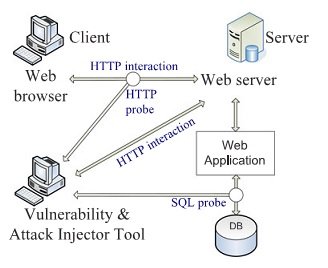
\includegraphics[width=0.7\linewidth]{Main/Fig2}}
\caption{VAIT setup}
\label{fig:Fig2}
\end{figure}

This is a key aspect of
the methodology to obtain the user interaction and the
results produced by such interaction for analysis, so they
can be used to prepare the attack. Therefore, the attack injection mechanism is aware of important inner workings of the
application while it is running. For example, this provides
insights on what piece of information supplied to a HTML
FORM is really used to build the correlated SQL query and
in which part of the query it is going to be inserted.The entire process is performed automatically, without human intervention.\\
\newline
%Example --can be removed if needed
For example,  consider the evaluation of an IDS: during the attack stage, when the IDS
inspects the SQL query sent to the database, the VAIT also
monitors the output of the IDS to identify if the attack has
been detected by the IDS or not. Only the
final results of the attack injection has to be collected, which also contains,the IDS detection output.\\
\section{ATTACK PROCEDURE}
The attack procedure mainly consist of 4 stages
\begin{enumerate}
	\item Preparation stage
	\item Vulnerability injection stage
	\item Attackload generation stage
	\item Attack stage
\end{enumerate}

\subsection{Preparation Stage}
In the preparation stage, the web application is interacted (crawled), executing all the functionalities that need to be tested (Fig.3.3). Both HTTP and SQL communications are captured by the two probes and processed for later use. The interaction with the web application is always done from the client's point of view.The outcome of this stage is the correlation of the input values, the HTTP variables that carry them and their respective source code files, and its use in the structure of the database queries sent to the back-end database (for SQLi) or displayed back to the web browser (for XSS).\\
\newline
Later, in the attack stage, the malicious activity applied is based on tweaking the values of the variables, which correspond to the text fields, combo boxes, etc., discovered in this preparation stage.
\begin{figure}[H]
\captionsetup{width=0.8\textwidth}
\begin{center}
\fbox{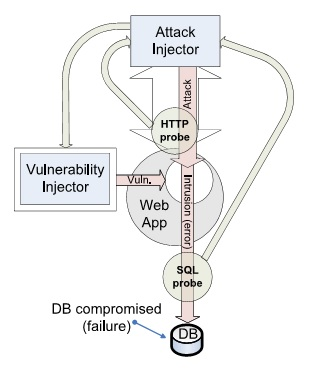
\includegraphics[scale=.8]{Main/Fig3}}
\caption{VAIT internal components}
 \label{fig:1}
\end{center}
\end{figure}

\subsection{Vulnerability Injection Stage}
 In the vulnerability injection stage, the vulnerabilities
are injected into the web application. For this purpose, it
needs information about which input variables carry relevant information that can be used to execute attacks to the web application. This stage starts by analyzing the
source code of the web application files searching for locations where vulnerabilities can be injected (Fig. 3.3). The injection of vulnerabilities is done by removing the protection of the target variables, like the call to a sanitizing
function. This process follows the realistic patterns resulting from the field study presented in [16]. Once it finds a
possible location, it performs a specific code mutation in
order to inject one vulnerability in that particular location.
The change in the code follows the rules derived from
[16], which are described and implemented as a set of
Vulnerability Operators.\\
\newline
The Vulnerability Operators are built upon a pair of
attributes: the Location Pattern and the Vulnerability Code
Change. The Location Pattern defines the conditions that
a specific vulnerability type must comply with and the
Vulnerability Code Change specifies the actions that
must be performed to inject this vulnerability, depending
on the environment where the vulnerability is going to
be injected.\\
\newline
The vulnerability and attack injection uses both
dynamic analysis and static analysis to gather the data
needed to apply the vulnerability operators. This analysis obtains not only the input variables (IV) that will be
part of an output variable (OV), but also the chain of variables in between. If the web application is secured, one
of the variables in the chain is sanitized or filtered
(Fig. 3.4). This variable is called target variable (TV),
because it is the one that the vulnerability injection stage
will try to make vulnerable by removing or changing the
protection scheme, according to the Vulnerability Operators. To inject a vulnerability using the Vulnerability
Operators, information about the target variable and the code location (CL) where it is sanitized or
filtered \{TV, CL\} is needed.
\begin{figure}
\centering
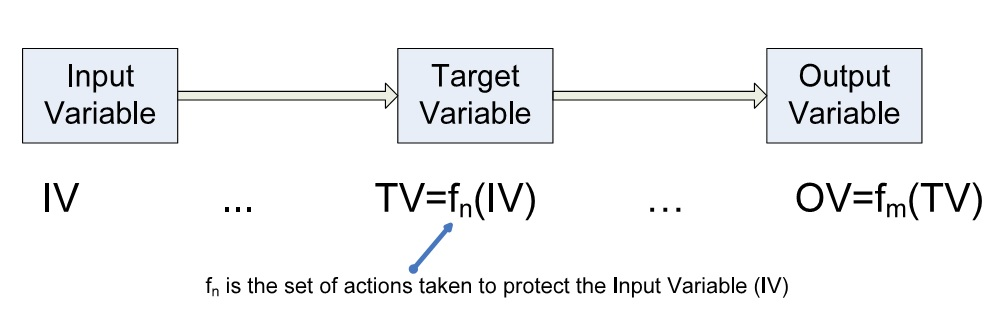
\includegraphics[width=0.7\linewidth]{Main/Fig4}
\caption{Chain of variables from input to output of the Web Application.}
\label{fig:Fig4}
\end{figure}\\
\newline
The preparation stage obtains  the pairs \{$ IV_{(dynamic analysis)}; OV_{(dynamic analysis)} $\}, which are the set of
input variables ($ IV_{(dynamic analysis)} $) whose values come from
the HTTP interaction or the SQL communication and their
mapping with output variables ($ OV_{(dynamic analysis)} $). On the other side, the vulnerability injector tool performs a static analysis on the source code and finds the input variables ($ IV_{(static analysis)} $) that are expected to be seen in the
output ($ OV_{(static analysis)} $) as part of the HTML response,
SQL queries, etc. It also provides the target variable
($ TV_{(static analysis)} $) and the code location ($ CL_{(static analysis)} $)
of the place in the file where the target variable is sanitized
or filtered. Overall, the static analysis provides the following set of attributes: \{$ IV_{(static analysis)}; OV_{(static analysis)} TV_{}(static analysis),$ \\$ CL_{(static analysis)}. $\}
%$ TV_{(static analysis); CL_{(static analysis)} $\}.
\\
\newline
The correlation of variables resulting from both static
and dynamic analysis originates a more precise set of locations where the Vulnerability Operators may be used. The
outcome of this correlation is an improved collection of
vulnerabilities that has a higher rate of exploitability by
the attack injection mechanism. The data must be provided
by the set of attributes that come from the static analysis
\{$ IV_{(static analysis)}, OV_{(static analysis)},$ \\ $ TV_{(static analysis)},
	CL_{(static analysis)} $\}, but improved by the pair of attributes
that come from the preparation stage \{$ IV_{(dynamic analysis)},
	OV_{(dynamic analysis)} $\} (Fig. 3.5). It considers the data from
the set of attributes \{$ IV_{(static analysis)}, OV_{(static analysis)},$
$TV_{(static analysis)}, $ \\ $CL_{(static analysis)} $\} but only whose pairs
\{IV$ _{}(static analysis), OV_{(static analysis)} $ \} are equivalent to any of
the \{$ IV_{(dynamic analysis)}, OV_{(dynamic analysis)} $ \}. The procedure to
process the data from dynamic and static analysis to obtain
the match outcome consisting of the pair of target variable
and code location \{TV, CL\} needed to apply the vulnerability operators
\begin{figure}
\centering
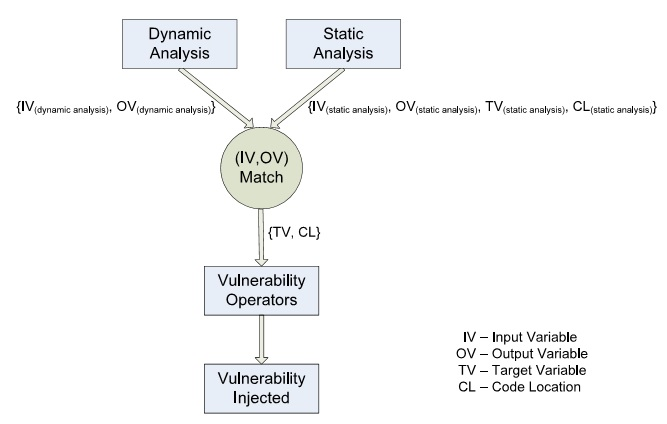
\includegraphics[width=0.7\linewidth]{Main/Fig5}
\caption{Using data from dynamic and static analysis to apply the vulnerability operators and inject a vulnerability.}
\label{fig:Fig5}
\end{figure}


\subsection{AttackLoad Generation Stage}
After having the set of copies of the web application
source code files with vulnerabilities injected, the collection of malicious interactions (attackloads) that will be used to attack each vulnerability need to be generated. This
is done in the attackload generation stage. The attackload
is the malicious activity data needed to attack a given vulnerability. This data is built around the interaction patterns derived from the preparation stage, by tweaking
the input values of the vulnerable variables.\\
\newline
The value that is assigned to the vulnerable variable, in
order to attack it, results from a fuzzing process. In this
process, the malicious value is obtained through the
manipulation of the data provided by the good values of
the vulnerable variable, the prefix $ (>,),`,``, \dots) $ and the suffix $ (<,–,\#,`,",\dots) $, the use of attackload strings and predefined functions (Fig. 3.6).The fuzzing process consists of combining the available collection of prefixes, attackload strings and suffixes.\\
\newline
\begin{figure}[H]
\centering
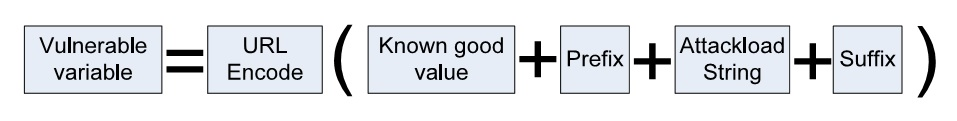
\includegraphics[width=0.7\linewidth]{Main/Fig6}
\caption{Fuzzer generated malicious variable value.}
\label{fig:Fig6}
\end{figure}
This stage also generates the payload footprints that
have a one to one relationship with the attack payloads.
The payload footprints are the expected result of the
attack. They can be the malicious SQL queries text sent to
the database, for the case of an SQLi attack; or the HTML
of the web application response, for the case of a XSS
attack. These payload footprints are fundamental, since
they are used to assess the success of the attack.

\subsection{Attack Stage}
In the attack stage, the web application is, once again, interacted. However, this time it is a ``malicious'' interaction since it consists of a collection of attack payloads in order to
exploit the vulnerabilities injected. The attack intends to
alter the SQL query sent to the database server of the web
application (for the case of SQLi attacks) or the HTML data
sent back to the user (for the case of XSS attacks).\\
\newline
The vulnerable source code files (from the vulnerability injection stage) are applied to the web application,
one at a time. Once again the two probes for capturing
the HTTP and SQL communications are deployed and
the collection of attackloads is submitted to exploit the vulnerabilities injected (Fig. 3.3). The interaction with the
web application is always done from the web client’s
point of view (the web browser) and the attackload is
applied to the input variables (the text fields, combo
boxes, etc., present in the webpage interface). At the end
of the attack, it is assessed for success. The
detection of the success of the attack is done by searching
for the presence of the payload footprint in the interaction
data (HTTP or SQL communications) captured by the two
probes. The process is repeated until all the injected vulnerabilities have been attacked.\\
\newline

\pagebreak


\section{VULNERABILITY \& ATTACK INJECTOR TOOL}

To demonstrate the feasibility of the proposed attack injection methodology, a prototype tool is developed ; Vulnerability \& Attack Injector Tool (VAIT).The VAIT prototype targets Linux, Apache, MySQL and PHP web applications, which is currently one of the most commonly used solution stack to develop web applications.\\
\newline
VAIT can injects vulnerabilities into the web application code and attacks them
in a seamlessly manner. As explained earlier, the process of attacking the web application
consists of 4 stages: the preparation stage, the vulnerability
injection stage, the attackload generation stage and the attack
stage (Fig 3.7). All this vulnerability and attack injection process will
be done with minimum human intervention.  The VAIT is
configured with the web application folder location. Then
the preparation stage is executed while the web application is being interacted. At the end, the vulnerability
injection stage automatically generates the vulnerabilities,
followed by the attackload generation stage that generates the attack payloads. At this point, the attack stage
can be executed to attack the vulnerabilities, collect the
results and calculate the attack success.
\begin{figure}
\centering
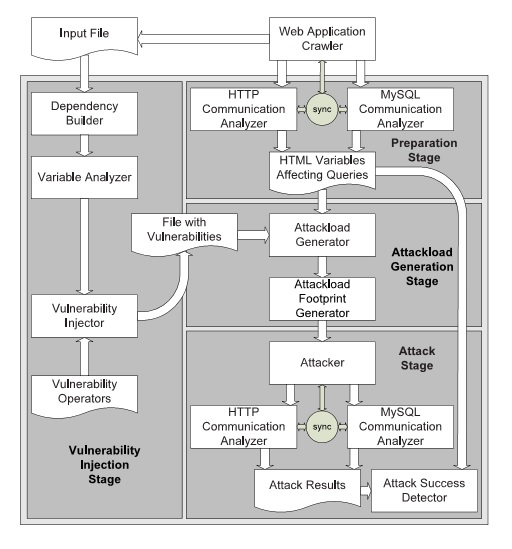
\includegraphics[width=0.7\linewidth]{Main/fig7}
\caption{VAIT architecture.}
\label{fig:fig7}
\end{figure}\\
\newline
During the preparation stage, the web application is executed. This interaction can be made either manually, by someone executing every web application procedure that should be tested, or automatically using an external tool, such as a web application crawler. During this interaction, the VAIT monitors the HTTP communication between the web browser and the web server and all the SQL communications going to and from the database server.\\
\newline
Monitoring is implemented using built-in proxies specifically developed for the HTTP and for the SQL communications. These proxies send a copy of the entire packet data
traversing them through the configured socket ports to the
HTTP Communication Analyzer and MySQL Communication
Analyzer components. Proxies run as independent processes
and threads, so they are relatively autonomous. To guarantee synchronization with other components of the VAIT, a
Sync mechanism was also built-in (Fig.3.7). The synchronism
is obtained by executing each web application interaction in
sequence without overlapping (i.e., without the common
use of simultaneous threads to speedup the process) and
gathering the precise time stamps of both the HTTP communication and respective SQL query. The interaction starts with the client actor (the browser of
the user of the web application) sending one HTTP request
that may lead SQL query requests to be sent to the database
server. Next, the database server responds to the SQL query
requests and sends the response back to the web application
server. Finally, the application server sends the HTTP
response back to the client actor. When the HTTP and SQL
proxies capture these serialized operations they also register
their time stamps, which allows the Sync mechanism to
group this distributed set of actions into meaningful causeeffect sequences.\\
\newline
The information gathered by both proxies contains the
structure of each webpage, the associated input variables, typical values and the associated SQL queries
where these variables are used. During this interaction,
the list of the web application files that are being run is
also sent to the integrated Vulnerability Injector as input
files. The vulnerability injector component is executed for each one, delivering the respective group of files with
injected vulnerabilities.\\
\newline
%\pagebreak
%\section{PROPOSED METHOD}
The current paper detects only the SQL injection(SQLi) attack and Cross Site Scripting (XSS) attacks. These two are the most common vulnerability found in the web application world.These two attacks attack the application data and the user information available with the system.But there are some other forms of attacks, targeting the server machine which runs these application itself.Attacks like Remote Code Execution (RCE) and File Inclusion (FI) attacks target the vulnerability in the web application and attacks the server machine instead of the web application. These kinds of attack can not only cause damage to the web application, but can even trouble the entire applications and services running on the main hardware and can even damage the normal working of the server operating system.\\
\newline
The VAIT tool proposed in the paper can be extended in order to identify the Remote Code Execution (RCE) and File Inclusion (FI) attack.Since these attacks does not necessarily need to have a communication with database, the attack cannot be identified by analyzing HTTP proxies and SQL proxies.Hence to identify these kinds of attack other methods have to be utilized.Static code analysis can identify these kinds of vulnerabilities easily but is very ineffective due to high false positive rates and low precision. One of the common way to identify these attacks are by analyzing the http data packets and performing a pattern matching analysis in it in order to identify erroneous patter.\\
\newline
A pattern mining approach based on dynamic analysis on input data and available information on method execution can easily identify attack injections of these kinds.So by utilizing a pattern mining algorithm and integrating it with the VAIT tool, the web application evaluation capability of the tool will be extended .




